\documentclass{article}
\usepackage{graphicx}
\usepackage[a4paper,margin=1in,footskip=0.25in]{geometry}
\usepackage{pdfpages}


\begin{document}


\title{Computer Forensics Laboratory Design}
\author{Jon Bakies \and Mitchell Dunn} 

\maketitle
\newpage

\tableofcontents
\newpage


\section{Laboratory Design}
\paragraph{} According to the NISTIR ``Forensic Science Laboratories: Handbook for Facility Planning, Design, Construction, and Relocation", a lab needs to be 700 to 1000 square feet per staff member.
The square footage per staff member approaches the low number of that threshold as the number of employees increases because shared spaces, such as reception areas and server rooms don't need to grow at the same rate as the number of employees.
With an estimated 8 staff members, this lab will require an approximate space of 6400 square feet to achieve the working goal of 800 service requests per year.

\subsection{Staff Breakdown}
\paragraph {Management - 1} 
\paragraph{} The laboratory manager is responsible for the well being of the lab.
To actively excel at their job, the manager must have general knowledge of law, computer forensics, and business.
This allows the manager to determine if the lab will be able to complete a service request based on current workload and legality. 
Most labs strive to have an ACLD/LAB accreditation status because it proves the lab follows a high standard of workplace protocol.
The manager must keep this in mind while creating policies for the rest of staff.
In order to keep evidence forensically sound a proper chain of custody record has to be met and the evidence has to be properly handled while being investigated.
These policies will not only improve the efficiency of the lab, but will also improve workplace ethics.
\paragraph{Lawyer - 1} 
\paragraph{} The Lawyer will act as a consult for the Computer Forensics staff to ensure all evidence is extracted legally and to verify the evidence is usable.

\paragraph{IT Specialist - 2}
\paragraph{}
The IT Specialists will focus on the internal network and security of the lab.
The IT Specialist should have 5 years experience as a system administrator, and be well versed in security.
The IT Specialists will be in charge of securing the hardware and evidence and managing access to the network hardware.
They should follow ACLD/LAB policies for lab and equipment security.
The IT Specialist will also act as a system administrator managing users, limiting communication between VLANs, hosting evidence to be easily accessed by authorized personnel, and maintaining the network for the Laboratory.

\paragraph{Computer Forensic Investigator - 5}
\paragraph{}
A computer forensic investigator should have the skills needed to extract evidence from a device in a non damaging and legal way.
It is important that the team of investigators are experienced in varying devices to enable the lab to accept a wide range of service requests.
Evidence and other information can be from from any electronic device, ranging from laptop and computers to mobile phones and game consoles.
All of these devices have their own operating system, meaning the investigator needs know how to work with multiple operating systems and software.
\subsection{Laboratory Layout}


\subsection{Figures}
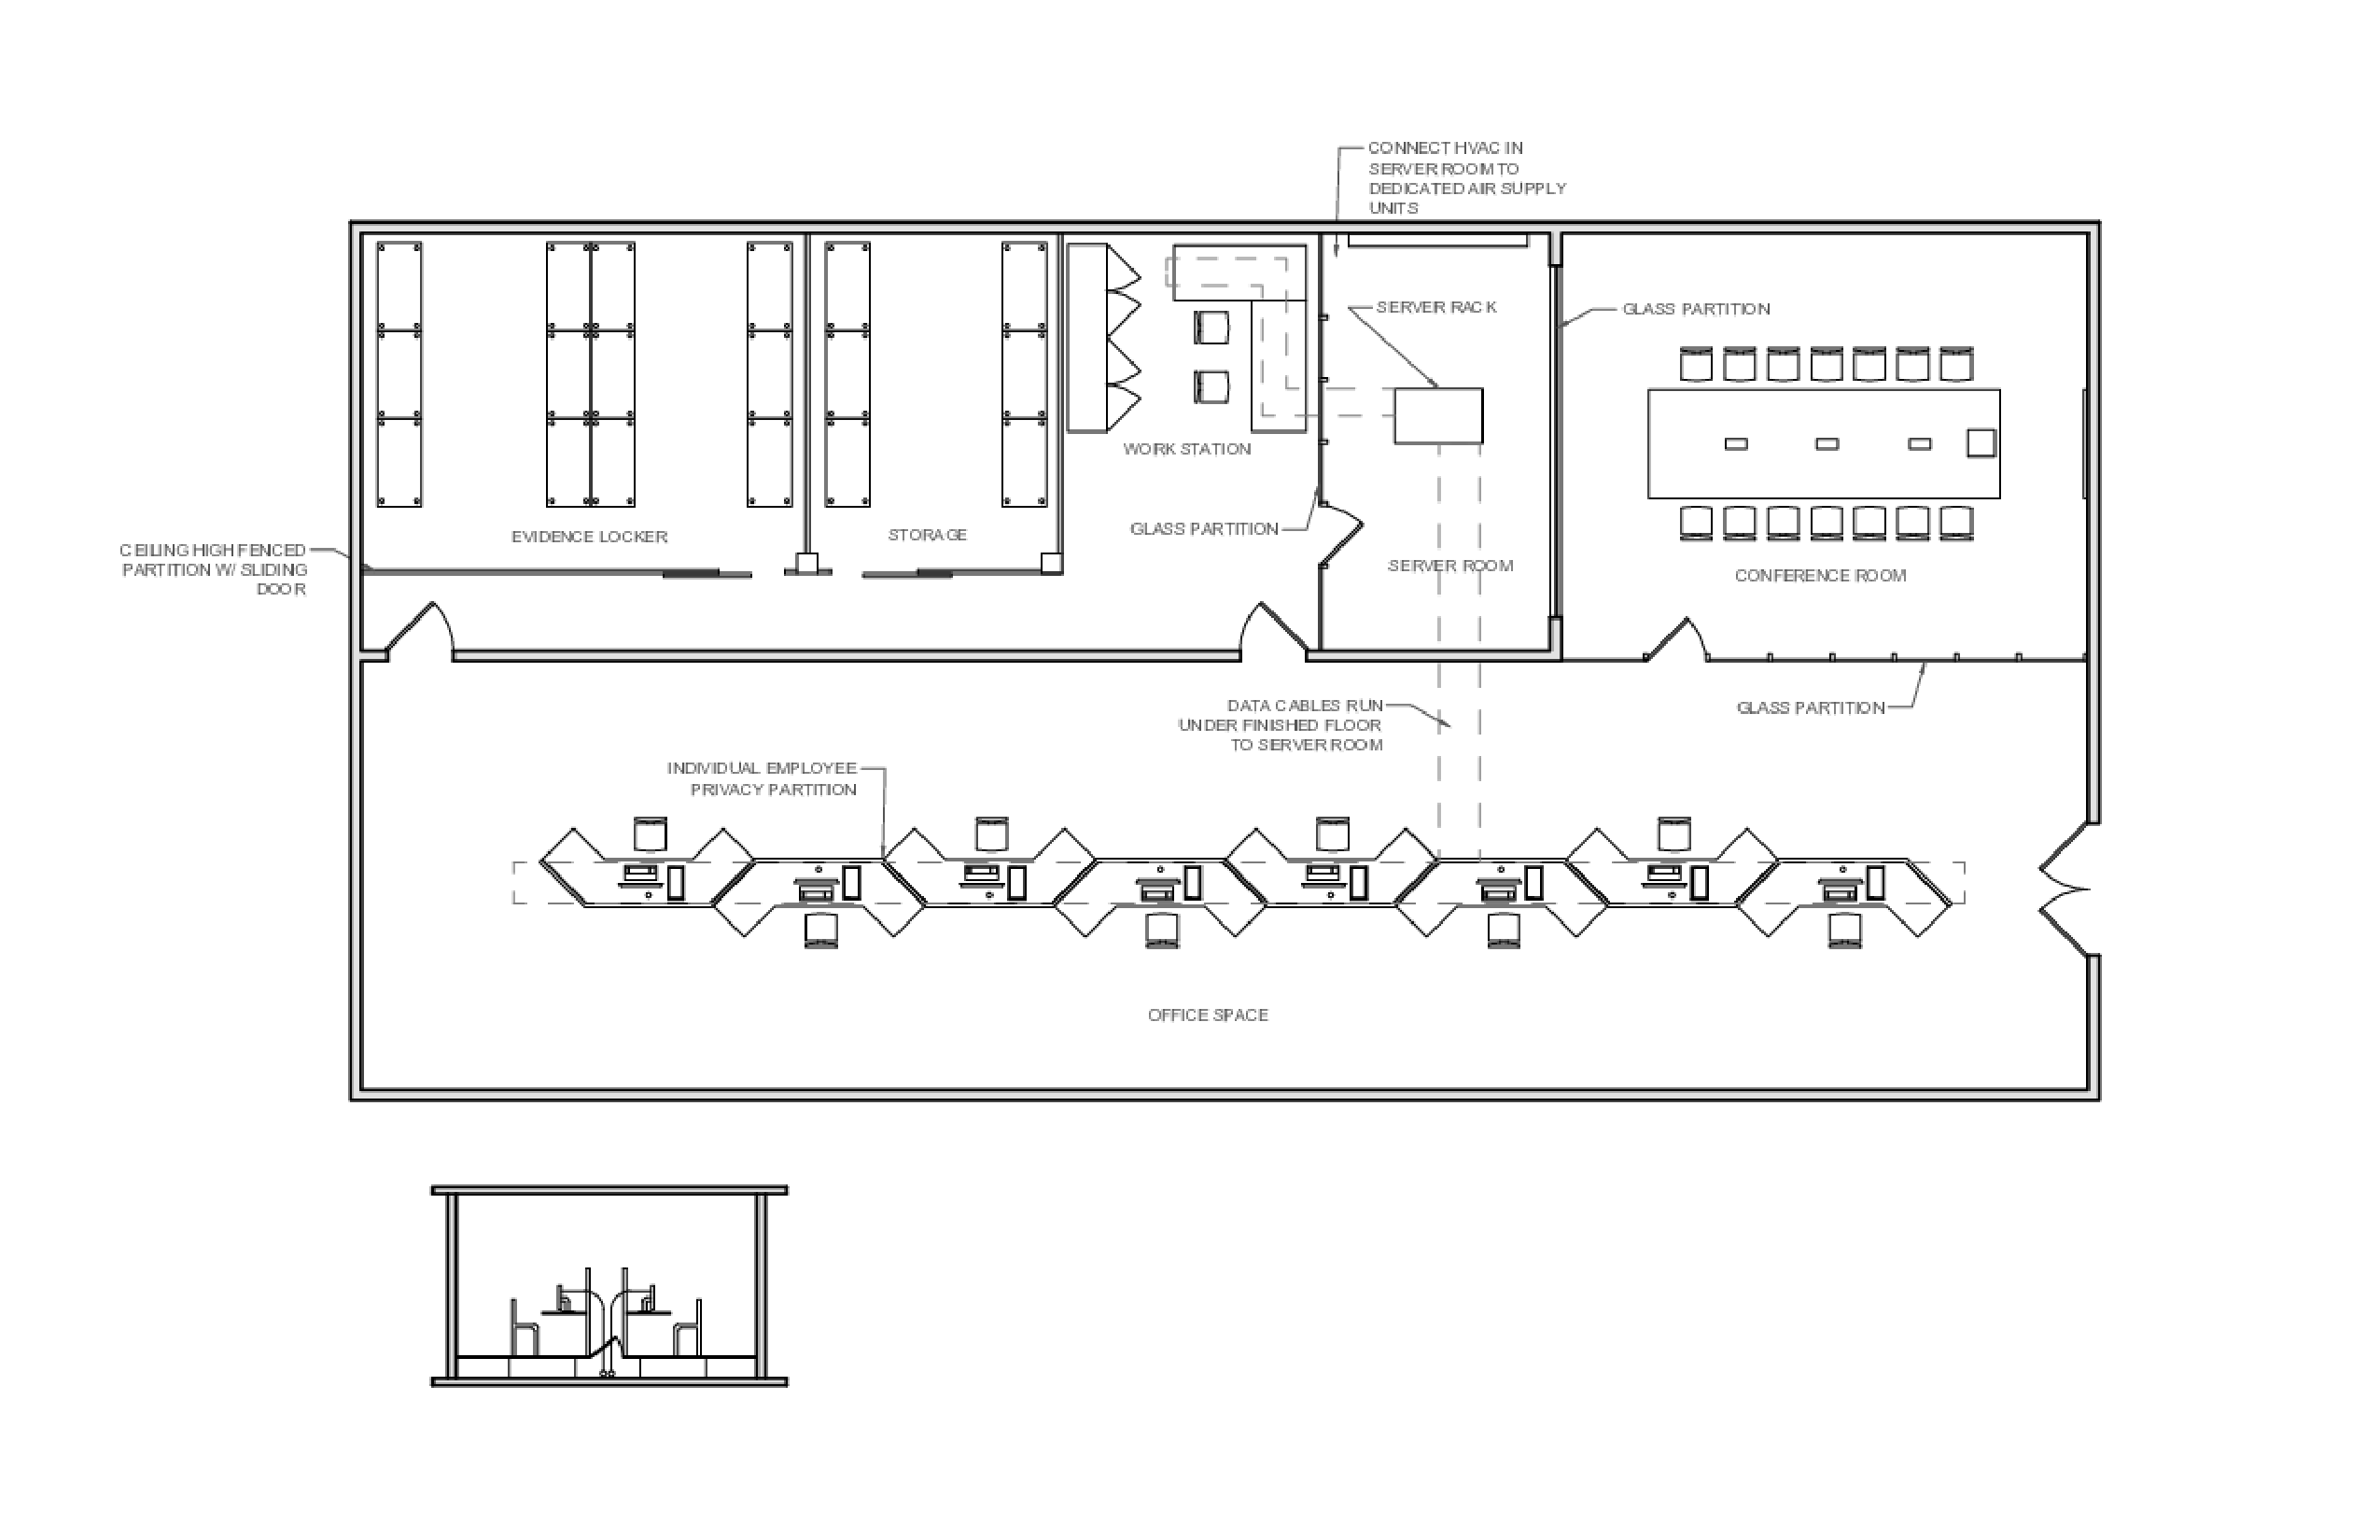
\includepdf[pages=-]{layout-thx-nick-millet-90.pdf}
\section{Hardware}
\subsection{Employee Laptops} 
\paragraph{}
All employees would receive Macbook Pros in order complete their daily tasks.
They would be provided thunderbolt docks in order to connect peripherals at their desk.
Which would allow them to use external displays, connect to the network with a cable, and setup mice and keyboards.
The 15 inch Macbook Pros are running seventh generation Intel processors and are highly capable of taking care of any task the investigators would need to do. 
If an investigator needs to run some analysis or search overnight they can use the virtual machine cluster at their will.
\paragraph{}
The employees can have additional hardware on their desk to make them more productive.
They can utilize Thunderbolt 3 docks to connect to as many peripherals as they like as well as charge their laptop.
These docks could connect to multiple high resolution screens. As well as a keyboard and mouse, a backup hard drive, and anything they find useful.

 
\subsection{Tools for Employees} 
\paragraph{}
Employees would have several tools available to them to use in their investigations.
These devices would be stored in the workspace next to the evidence locker.
\begin{itemize}
\item Hard Drive Write Blockers for all the different hard drive connectors
\item 
\end{itemize} 
% list shit here

\subsection{Server Rack}
\subsubsection{Power Supply}
\paragraph{}
The power supply to the server rack should be through an uninterruptible power supply (UPS) in order to ensure that the power supplied is clean and backed up by a battery.
The UPS should have enough capacity to run for the time it takes to start a diesel generator to take over as the power supply.
The diesel generator should have monthly testing, as well as the power supply failover operation.
Each system in the rack should have two power supplies to help guarantee uptime.
Each leg of the system should be plugged into a different rack mounted power supply to allow a power supply failure.
 
\subsubsection{Networking}
\paragraph{}
The networking would be simple, one 48 port switch would be sufficient for the entire network.
And the connection to the ISP would be connected to a Router/Firewall box.
The connection to the ISP should be fiber and have an uplink of at least 500Mbps to ensure that employees can connect remotely and download large files without saturating the link for a long time.
A second connection to a different ISP should be considered, to be used as a failover in case of maintenance to the first ISP.
To improve security further on the ISP link a Network Detection and Response, such as RSA's NetWitness system would be running on the internal virtual machine cluster described below.
Each virtual machine would need three uplinks, one to the employee local area network, one to the Storage area network, and one link for VMWare.
These networks will be isolated from each other using VLANs in order to enhance security.
Other VLANs could be implemented to further isolate network devices like IP Cameras and smart door locks to prevent people from directly accessing and potentially compromising them.
A wifi access point connected to the switch and employees would authenticate to Active Directory to ensure only employee devices are connecting.
This wifi would be most useful in the conference room while the employees are away from their workstations.
Another vlan and separate wireless network, even on the same physical access point, with a password could also be provided to convenience the employees by providing wifi to their personal devices (e.g. personal cellphones).
The second network would have very strict firewall rules and would not pass traffic to any of the other networks.
At the employees desks would be a wired connection for more reliable networking to the employees workstations. 
Small switches every few desks powered using power over ethernet would limit the amount of cables needed to run all the way back to the server rack to be connected to the network.
The ethernet network can be secured using 802.1x so that no unauthorized computers could access the network. 



\subsubsection{Virtual Machine Cluster}
\paragraph{}
The purpose of the virtual machine cluster is to provide investigators with multiple computers in the most convenient way possible.
Since investigators should have access to any operating system they could would need at any time instantly, it is expected that each investigator will have three to five virtual machines at any time.
In addition to investigators the IT staff might also want to run some virtual machines for their convenience.
This cluster will also provide infrastructure for internal and external services.
Internal services would include Active Directory, samba/NFS/FTP sites, etc.
Active Directory would be the central authentication for all the services.
Each server in the cluster would be dual socket motherboards to provide the high amount of compute power needed to run all the virtual machines.
The servers would also be installed with high capacity error correcting memory to a lot of RAM can b allocated to virtual machines working with disk images.
If the capacity allows it VMWare's high availability features can be leveraged to run multiple copies of the same virtual machine for critical infrastructure like the Windows Domain Controller in order to ensure that even if a physical host powers off unexpectedly the domain controller would continue to operate and employees are not interrupted.
For cases where video processing is involved graphics cards can be installed on the virtual machine hosts and using PCI passthrough to attach graphics cards to the virtual machines to greatly enhance their video performance.
This would allow investigators to comforatbly work from their laptop and still have the benefits of full size, powerful graphics cards.

\subsubsection{Storage}
\paragraph{} 
In order to be running many virtual machines the storage needs to be very performant Using all solid state hard drives in an array will achieve this.
Using a separate VLAN for the storage to reach the virtual machine cluster with 10Gb ethernet would allow enough bandwidth to run as many virtual machines 
With all the bandwidth on the many solid state drives the server would be able to perform enough IOPs to run all of the virtual machines at the same time.

\subsubsection{Remote Storage}
\paragraph{}
Remote storage could be secured at a remote colocation facility in order to facilitate the use of offsite backups for employee computers and evidence that is critical to a case. 
Many dedicated storage systems have features built and this can be leveraged to easily send rolling backups to the remote location. 
This can be done at a late at night and a pace that does not affect any of the few systems that are normally running that late. 

\section{Software}
\subsection{VMWare Fusion} 
\paragraph{}
VMWare fusion would allow employees to connect to different virtual machines easily.
The software would allow seamless integration with the employees mouse and keyboard. 
Features like shared clipboard and being able to drag and drop files between the host and guest.

\end{document}
